
\section*{Introduction}

Le chapitre précédent était consacré à la mise en place des éléments de base de notre système. Nous y avons développé l'authentification et la gestion des utilisateurs avec leurs rôles et permissions. Nous avons aussi travaillé sur la gestion des clients et le processus de traitement des demandes d'inscription. L'ensemble de ces fonctionnalités a été testé et validé.
\newline Dans ce chapitre, nous passons au développement du cœur métier. Il s'agit principalement des contrats de maintenance avec leurs SLA, des projets et de leurs équipes, ainsi que de l'historique qui assure la traçabilité de toutes les modifications.
% ─────────────────────────────────────────────────────────────────────────────
% SECTION 1 : BACKLOG DU SPRINT 2
% ─────────────────────────────────────────────────────────────────────────────
\section{Sprint Planning Meeting }
La réunion de planification du deuxième sprint nous a permis de définir les objectifs à atteindre durant les trois prochaines semaines. Nous avons sélectionné les user stories prioritaires et estimé l'effort nécessaire pour chacune d'elles. Cette étape est importante pour que toute l'équipe comprenne bien le travail à réaliser.
\newline
\subsection{Objectif du Sprint}
Ce sprint vise à développer les fonctionnalités essentielles du système. L'objectif principal est de mettre en place la gestion des contrats de maintenance et d'assurer le suivi des engagements de service à travers leurs SLA, de faciliter la collaboration via l'affectation des équipes aux projets, et de garantir la traçabilité complète des opérations effectuées.
\subsubsection{Backlog du deuxième sprint}
\label{sec:backlog_sprint2}

Le tableau ci-dessous présente le Sprint Backlog détaillé avec les descriptions techniques et l'effort estimé pour chaque user story.
\newline
\textbf{1 : Effort faible, 2 : Effort moyen, 3 : Effort élevé}

\rowcolors{0}{}{}
\arrayrulecolor{black}
\renewcommand{\arraystretch}{1.3}
\small

\begin{longtable}{|C{1cm}|m{6.5cm}|m{7cm}|C{1cm}|}
\hline
\textbf{ID US} & \textbf{User Story} & \textbf{Description technique} & \textbf{Effort} \\
\hline
\endfirsthead

    \hline

\endhead

\hline
\endfoot

\hline
\endlastfoot
\multicolumn{4}{|l|}{\cellcolor{blue!20}\textbf{Epic 5 - Gestion des Clients}} \\
\hline
 US17 & En tant qu'\textbf{administrateur}, je souhaite créer un profil client afin de centraliser ses informations. &
\vspace{2mm}
\begin{itemize}[nosep, left=0pt, label={$\bullet$}]
\item Développer l’endpoint POST /clients pour orchestrer la création simultanée du compte CLIENT et du profil entreprise associé.  
\item  Implémenter un service de récupération automatique de logo (LogoService) établi sur le nom de la société
\item Intégrer une logique de gestion des projets historiques pour associer des projets passés, des chefs de projets et des membres d'équipe au nouveau client
\item Réaliser l'interface de formulaire
\end{itemize} & 1 \\
\hline

US18 & En tant qu’administrateur, je souhaite consulter la liste des clients  afin de visualiser les clients existants. &
\vspace{2mm}
\begin{itemize}[nosep, left=0pt, label={$\bullet$}]
\item Développer l’endpoint GET /clients intégrant une logique de filtrage RBAC.
\item Réaliser une interface de visualisation
\end{itemize} & 2 \\
\hline
US19 & En tant qu'\textbf{administrateur}, je souhaite consulter le profil détaillé d'un client afin de visualiser toutes ses informations. &
\begin{itemize}[nosep, left=0pt, label={$\bullet$}]
\item Développer l’endpoint GET /clients/:id pour récupérer les informations du client.
\item Réaliser une interface de profil structurée.
\item Développer des composants spécifiques pour l'affichage des informations secondaires       
\end{itemize} & 1 \\
\hline
US20 & En tant qu'\textbf{administrateur}, je souhaite modifier les informations d'un client afin de maintenir des données à jour. &
\begin{itemize}[nosep, left=0pt, label={$\bullet$}]
\item Développer l’endpoint PATCH /clients/:id permettant la mise à jour des informations des clients. 
\item Développer des contrôles d'intégrité côté serveur pour valider les formats de données.
\item Réaliser une interface d'édition fluide.
\end{itemize} & 2 \\
\hline
US21 & En tant qu'\textbf{administrateur}, je souhaite activer et désactiver un compte client afin de contrôler l'accès. &
\begin{itemize}[nosep, left=0pt, label={$\bullet$}]
\item Développer les endpoints de changement de statut (POST /desactiver, POST /reactiver)
\item Implémenter la vérification pour bloquer l'opération si le client possède des contrats actifs, des demandes en attente ou des tickets non résolus.  
\item Intégrer le EmailService pour l'envoi automatique de notifications transactionnelles de changement de statut.                           
\end{itemize} & 3 \\
\hline

US22 & En tant qu'\textbf{administrateur}, je souhaite imprimer l'annuaire d'un client afin de disposer d'une version papier. &
\begin{itemize}[nosep, left=0pt, label={$\bullet$}]
\item Développer l'endpoint POST /clients pour créer un client avec validation des données
\end{itemize} & 1 \\
\hline

US23 & En tant qu'\textbf{administrateur}, je souhaite créer un projet rattaché à un client afin d'organiser les interventions. &
\vspace{2mm}
\begin{itemize}[nosep, left=0pt, label={$\bullet$}]
\item Développer l'API de création avec validation des données
\item Gérer les relations projet-client et envoyer les notifications aux membres de l'équipe
\item Créer le formulaire multi-étapes avec sélection guidée 
\end{itemize} & 3 \\
\hline 
US24 & En tant qu'\textbf{administrateur}, je souhaite consulter la liste des projets afin de piloter l'activité. &
\vspace{2mm}
\begin{itemize}[nosep, left=0pt, label={$\bullet$}]
\item Développer l'API de consultation avec filtres et contrôler l'accès selon le rôle
\item Récupérer les données enrichies et paginer les résultats
\item Créer l'interface avec tableau, filtres avancés et proposer les vues multiples (liste/cartes/Kanban)
\end{itemize} & 2 \\
\hline
US25 & En tant qu'\textbf{administrateur}, je souhaite affecter des développeurs à un projet afin de constituer l'équipe. &
\vspace{2mm}
\begin{itemize}[nosep, left=0pt, label={$\bullet$}]
\item Développer l'API d'affectation avec workflow de validation
\item Calculer automatiquement la disponibilité et envoyer les notifications en temps réel à chaque étape
\item Créer les interfaces de gestion d'équipe avec suivi des propositions
\end{itemize} & 3 \\
\hline
US26 & En tant que \textbf{membre d'équipe}, je souhaite consulter les informations du projet afin de comprendre le contexte. &
\vspace{2mm}
\begin{itemize}[nosep, left=0pt, label={$\bullet$}]
\item Développer l'API de détail avec contrôle d'accès 
\item Créer la page détaillée organisée en sections avec les informations du projet
\end{itemize} & 1 \\
\hline


% Epic 2: Gestion des utilisateurs
\multicolumn{4}{|l|}{\cellcolor{blue!20}\textbf{Epic 7 -Gestion des Contrats}} \\
\hline

US28 & En tant qu’administrateur, je souhaite créer un contrat de maintenance afin de formaliser les engagements de service avec le client. & 
\vspace{2mm}
\begin{itemize}[nosep, left=0pt, label={$\bullet$}]
\item Développer l'API de création avec deux modes : formulaire manuel et upload PDF avec extraction automatique (pdf-parse + regex)
\item Implémenter l'extraction des données du PDF (référence, dates, montants, SLA, client, projet) et résolution automatique en base
\item Créer l'interface avec choix du mode, pré-remplissage automatique du formulaire et stockage avec hashage anti-doublon
\end{itemize}
& 2 \\
\hline

US29 & En tant qu’administrateur, je souhaite consulter la liste des contrats afin de suivre les engagements contractuels. & 
\vspace{2mm}
\begin{itemize}[nosep, left=0pt, label={$\bullet$}]
\item Développer l'API de consultation avec filtres avancés et contrôle d'accès RBAC
\item Récupérer les données enrichies avec pagination
\item Créer l'interface avec tableau, filtres, badges de statut et actions rapides (voir, modifier, archiver)
\end{itemize}
& 3 \\
\hline

US30 & En tant qu’administrateur, je souhaite recevoir des alertes avant l’expiration des contrats afin d’anticiper les renouvellements & 
\vspace{2mm} 
\begin{itemize}[nosep, left=0pt, label={$\bullet$}]
\item Développer le système d'alertes automatiques (30, 15, 7 jours avant expiration) avec CRON job
\item Envoyer les notifications par email et in-app avec détails du contrat
\item Créer l'interface d'alertes avec liste des contrats à renouveler
\end{itemize}
& 2 \\
\hline

US31 & En tant qu’administrateur, je souhaite archiver un contrat afin de conserver l’historique. & 
\vspace{2mm}
\begin{itemize}[nosep, left=0pt, label={$\bullet$}]
\item Développer l'API d'archivage avec vérifications (pas de demandes en cours, confirmation requise)
\item Gérer le changement de statut et conserver les données historiques avec motif d'archivage
\item Créer le dialogue de confirmation 
\end{itemize}
 & 3 \\
\hline

US32 & En tant que client, je souhaite demander la résiliation de mon contrat afin d’interrompre le service.& 
\vspace{2mm}
\begin{itemize}[nosep, left=0pt, label={$\bullet$}]
\item Développer l'API de demande de résiliation avec workflow (demande → validation admin → résiliation)
\item Envoyer les notifications aux administrateurs et gérer le statut du contrat
\item Créer le formulaire de demande avec motif obligatoire
\end{itemize}
 & 1 \\
\hline

US33 & En tant qu’administrateur, je souhaite résilier un contrat afin de l’interrompre avant terme. & 
\vspace{2mm} 
\begin{itemize}[nosep, left=0pt, label={$\bullet$}]
\item Développer l'API de résiliation avec validation
\item Gérer le changement de statut et notifier le client par email
\item Créer le dialogue de résiliation avec confirmation 
\end{itemize}
& 2 \\
\hline

\hline



US35 & En tant que chef de projet, je souhaite consulter les contrats dans un calendrier afin de visualiser les dates d’expiration& 
\vspace{2mm} 
\begin{itemize}[nosep, left=0pt, label={$\bullet$}]
\item Développer l'API de récupération des contrats avec dates (début, expiration) filtrées par période
\item Calculer les indicateurs (contrats expirant bientôt, contrats actifs) pour la vue calendrier
\item Créer la vue calendrier avec affichage des contrats par mois et code couleur selon le statut

\end{itemize}
& 1 \\
\hline
 US36 & En tant que \textbf{client}, je souhaite soumettre un retour d'expérience à l'expiration de mon contrat afin d'exprimer ma satisfaction.&
 \vspace{2mm} 
\begin{itemize}[nosep, left=0pt, label={$\bullet$}]
\item Développer l'endpoint POST /contrats/:id/feedback pour enregistrer la note, le commentaire et l'intention de renouvellement dans FeedbackExpirationContrat
\item Implémenter une logique de déclenchement automatique de notification aux administrateurs si le client souhaite renouveler
\item Réaliser le formulaire de feedback côté client avec affichage conditionnel selon le statut du contrat 

\end{itemize}
& 1 \\
\hline
US37 & En tant qu'\textbf{administrateur}, je souhaite générer un PDF formaté du contrat afin de le partager avec le client.&
 \vspace{2mm}
 &2 \\
 \hline
% Epic 3: Gestion des rôles et permissions
\multicolumn{4}{|l|}{\cellcolor{blue!20}\textbf{Epic 14 - Consulter journal d'activité}} \\
\hline

US95 & En tant qu’administrateur, je souhaite consulter l’historique complet de toutes les actions afin d’assurer la traçabilité. & 
\vspace{2mm}
\begin{itemize}[nosep, left=0pt, label={$\bullet$}]
\item Développer l'API de consultation avec pagination, filtres avancés et recherche textuelle
\item Récupérer les logs enrichis avec informations utilisateur et statistiques (taux de succès, actions fréquentes)
\item Créer l'interface avec tableau filtrable, timeline, graphiques de statistiques et vue détaillée par entité
\end{itemize}
 & 3 \\
\hline

US96 & En tant qu’administrateur, je souhaite exporter les logs d’audit afin de répondre aux exigences de conformité. & 
\vspace{2mm} 
\begin{itemize}[nosep, left=0pt, label={$\bullet$}]
\item Développer l'API d'export avec formats CSV et JSON, filtres personnalisables et limite de 10 000 enregistrements
\item Implémenter le nettoyage automatique des logs anciens
\item Créer l'interface d'export avec sélection de format, prévisualisation et téléchargement direct
\end{itemize}
& 2 \\
\hline

\end{longtable}


% ─────────────────────────────────────────────────────────────────────────────
% SECTION 2 : ANALYSE
% ─────────────────────────────────────────────────────────────────────────────

\section{Analyse}

\label{sec:analyse_sprint2}

\subsection{Diagramme des cas d'utilisation du deuxième sprint}

La figure ci-dessous présente le diagramme de cas d’utilisation du deuxième sprint : 

\begin{figure}[H]
        \centering
        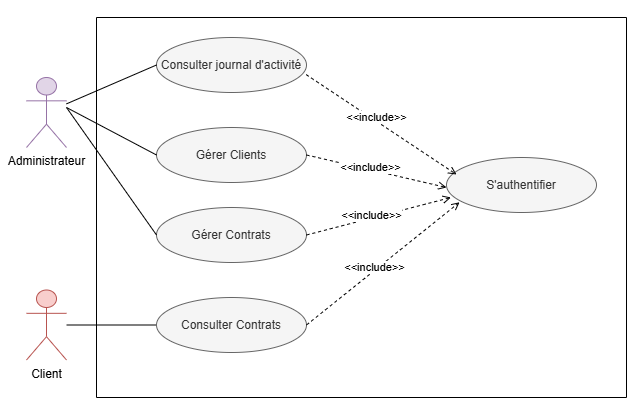
\includegraphics[width=0.85\textwidth,height=0.75\textheight,keepaspectratio]{Images/diagramme cas utilisation sprint2.png}
        \caption{Diagramme des cas d'utilisation du deuxième sprint}
        \label{fig:use_case_sprint2}
\end{figure}
Nous allons accompagner les cas d'utilisation d'un texte descriptif pour expliquer le scénario de chaque cas ainsi que ses exceptions.



\subsection{Analyse de la fonctionnalité « Gérer Contrats »}

Dans cette partie, nous allons présenter les cas d’utilisation relatifs à la gestion des Contrats afin de comprendre
les principales fonctionnalités du système, ce qui permet d’avoir une vue globale des interactions.
\subsubsection{Raffinement de cas d'utilisation « Gérer Contrats »}
Au cours de cette partie, nous allons analyser chaque cas d’utilisation raffiné pour le cas de gestion des Contrats :

\begin{figure}[H]
        \centering
        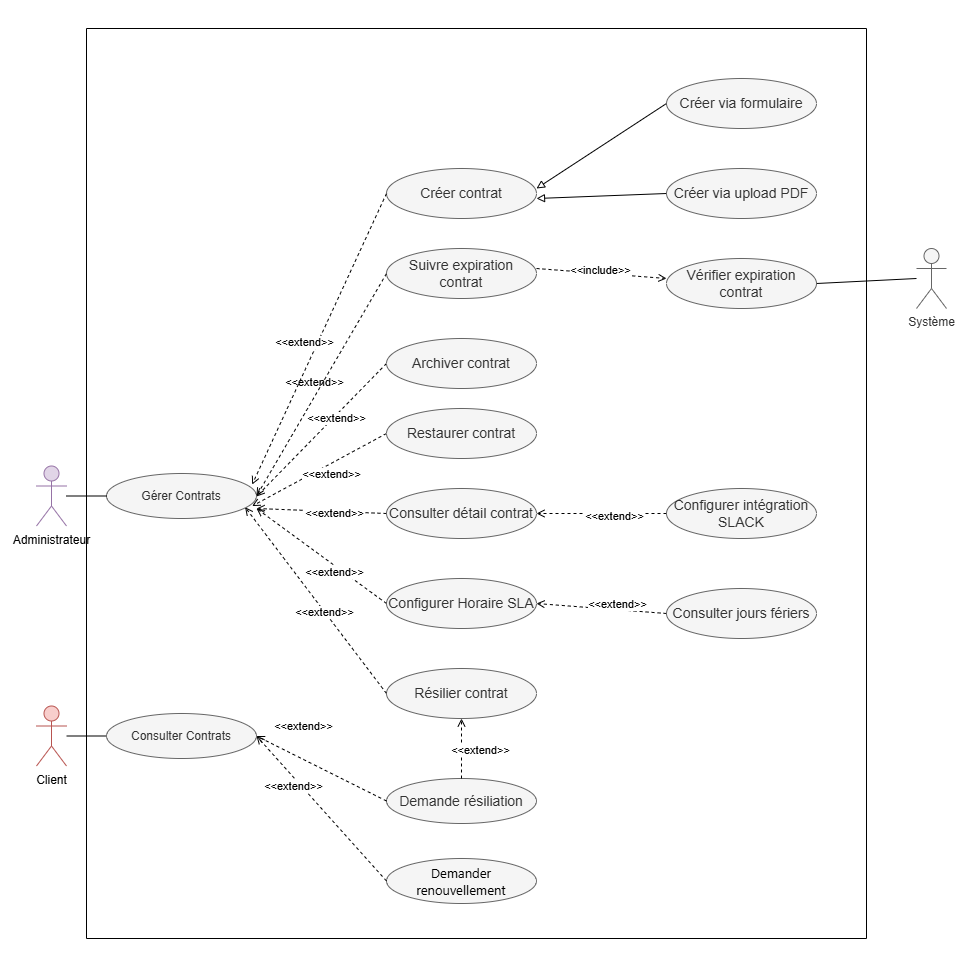
\includegraphics[width=0.9\textwidth,height=0.75\textheight,keepaspectratio]{Images/Diagramme de cas utilisation gestion contrat.png}
        \caption{Diagramme des cas d'utilisation « Gérer Contrats »}
        \label{fig:gerer_contrats}
\end{figure}

\subsubsection{Description textuelle de cas d'utilisation « Créer contrat »}
\vspace{-0.3cm}
\begin{table}[h]
\centering
\footnotesize
\renewcommand{\arraystretch}{1}

\begin{tabular}{|p{4.5cm}|p{12cm}|}
\hline
\textbf{Nom du cas d'utilisation} & Créer un contrat \\
\hline
\textbf{Acteurs} & Administrateur \\
\hline
\textbf{Préconditions} & 
L'utilisateur est authentifié.\newline
L'utilisateur possède la permission de créer des contrats. \newline
La liste des contrats est accessible.\\
\hline
\textbf{Postconditions} & 
  Le contrat est enregistré avec le statut ACTIF et une référence générée automatiquement.\newline
  Le contrat est visible dans la liste des contrats et lié au client sélectionné.\\
\hline
\textbf{Scénario principal} & 
\begin{minipage}[t]{\linewidth}
\begin{enumerate}[label=\arabic*., leftmargin=*]
 \item L'administrateur clique sur « Nouveau » depuis la liste des contrats.
    \item Le système propose deux modes : \textit{Saisie manuelle} ou \textit{Import PDF}.
    \item L'administrateur sélectionne \textit{Saisie manuelle} et confirme.
    \item L'administrateur renseigne les informations du contrat : client, projet, dates, montant, devise et taux de TVA.
    \item L'administrateur configure le niveau de service (SLA) avec les délais par priorité.
    \item L'administrateur valide le formulaire.
    \item Le système enregistre le contrat et redirige vers la liste des contrats.
  
\end{enumerate}
\vspace{2pt}
\end{minipage} \\
\hline
\textbf{Scénarios alternatifs} & 
\begin{itemize}[nosep,leftmargin=0.8cm,topsep=0pt,itemsep=2pt, label=$\bullet$]
    \item  L'administrateur choisit le mode 
    \textit{Import de document} et dépose un fichier PDF. Le système 
    extrait automatiquement les données et pré-remplit le formulaire. 
    L'administrateur vérifie les données, sélectionne le client et le 
    projet, puis valide.

\end{itemize} \\
\hline
\textbf{Scénarios d'exception} & 
\begin{itemize}[nosep,leftmargin=0.8cm,topsep=0pt,itemsep=2pt, label=$\bullet$]
         \item  Le système détecte qu'un contrat actif existe déjà pour ce client/projet et affiche un message de blocage.
    \item  Le système détecte que le client, les dates ou le montant ne sont pas renseignés et affiche un message d'erreur.
    \item Le système détecte que la date de début est antérieure à aujourd'hui ou que la date d'expiration est antérieure ou égale à la date de début et affiche un message d'erreur.
    \item Le système détecte que le montant saisi est nul ou non numérique et affiche un message d'erreur.
  
\end{itemize} \\
\hline
\end{tabular}
\caption{Description textuelle « Créer contrat »}
\end{table}
\vspace{-0.3cm}


\subsubsection{Description textuelle de cas d'utilisation « Archiver contrat »}
\vspace{-0.3cm}
\begin{table}[H]
\centering
\footnotesize
\renewcommand{\arraystretch}{1}

\begin{tabular}{|p{4.5cm}|p{12cm}|}
\hline
\textbf{Nom du cas d'utilisation} & Archiver un contrat \\
\hline
\textbf{Acteurs} & Administrateur \\
\hline
\textbf{Préconditions} &
  L'utilisateur est authentifié.\newline
  L'utilisateur possède la permission d'archiver des contrats.\newline
  Le contrat est expiré et non encore archivé.\\
\hline
\textbf{Postconditions} &
  Le contrat est marqué comme archivé et n'apparaît plus dans la 
  liste principale.\newline
  Le motif d'archivage est enregistré et associé au contrat.\\
\hline
\textbf{Scénario principal} &
  \begin{minipage}[t]{\linewidth}
  \begin{enumerate}[label=\arabic*., leftmargin=*]
    \item L'administrateur sélectionne un contrat expiré depuis la liste.
    \item L'administrateur clique sur « Archivage définitif » dans le 
    menu contextuel.
    \item Le système affiche un dialogue de confirmation demandant un 
    motif d'archivage.
    \item L'administrateur saisit un motif et confirme.
    \item Le système archive le contrat et met à jour la liste.
  \end{enumerate}
  \vspace{2pt}
  \end{minipage} \\
\hline
\textbf{Scénarios alternatifs} &
  \begin{itemize}[nosep,leftmargin=0.8cm,topsep=0pt,itemsep=2pt, label=$\bullet$]
    \item  L'administrateur sélectionne 
    plusieurs contrats expirés et clique sur « Archiver la sélection ». 
    Le système archive tous les contrats éligibles et affiche le nombre 
    de contrats archivés avec succès.
  \end{itemize} \\
\hline
\textbf{Scénarios d'exception} &
  \begin{itemize}[nosep,leftmargin=0.8cm,topsep=0pt,itemsep=2pt, label=$\bullet$]
    \item Le système détecte que le contrat 
    n'est pas encore expiré et bloque l'action d'archivage.
    \item  Le système détecte que le motif 
    saisi contient moins de 10 caractères et désactive le bouton de 
    confirmation.
  \end{itemize} \\
\hline
\end{tabular}
\caption{Description textuelle « Archiver contrat »}
\end{table}
\vspace{-0.3cm}

\subsubsection{Description textuelle de cas d'utilisation « Configurer intégration Slack »}
\vspace{-0.3cm}
\begin{table}[H]
\centering
\footnotesize
\renewcommand{\arraystretch}{1}
\begin{tabular}{|p{4.5cm}|p{12cm}|}
\hline
\textbf{Nom du cas d'utilisation} & Configurer intégration Slack \\
\hline
\textbf{Acteurs} & Administrateur \\
\hline
\textbf{Préconditions} &
  L'administrateur est authentifié.\newline
  Un contrat est sélectionné.\\
\hline
\textbf{Postconditions} &
  La configuration Slack est enregistrée et liée au contrat.\newline
  Les notifications sont actives selon les préférences choisies.\\
\hline
\textbf{Scénario principal} &
  \begin{minipage}[t]{\linewidth}
  \begin{enumerate}[label=\arabic*., leftmargin=*]
    \item L'administrateur clique sur « Intégration Slack » depuis 
    le menu contextuel du contrat.
    \item Le système affiche le dialogue de configuration Slack.
    \item L'administrateur saisit l'URL du webhook et le canal Slack.
    \item L'administrateur configure les types de notifications 
    souhaités : ticket créé, mise à jour, résolu, critique seulement.
    \item L'administrateur clique sur « Configurer ».
    \item Le système enregistre la configuration et l'associe 
    au contrat.
  \end{enumerate}
  \vspace{2pt}
  \end{minipage} \\
\hline
\textbf{Scénarios alternatifs} &
  \begin{itemize}[nosep,leftmargin=0.8cm,topsep=0pt,itemsep=2pt, label=$\bullet$]
    \item
    Le système détecte qu'une configuration Slack existe déjà pour 
    ce contrat et pré-remplit le formulaire. L'administrateur modifie 
    les champs souhaités et clique sur « Mettre à jour ».
    \item  Après sauvegarde, 
    l'administrateur clique sur « Tester ». Le système envoie un 
    message de test sur le canal Slack configuré.
    \item L'administrateur 
    clique sur le bouton de suppression. Le système supprime la 
    configuration Slack du contrat.
  \end{itemize} \\
\hline
\textbf{Scénarios d'exception} &
  \begin{itemize}[nosep,leftmargin=0.8cm,topsep=0pt,itemsep=2pt, label=$\bullet$]
    \item  Le système détecte 
    que le webhook URL ou le canal ne sont pas renseignés et affiche 
    un message d'erreur.
    \item Le système détecte que le webhook 
    URL est invalide lors du test et affiche un message d'erreur.
  \end{itemize} \\
\hline
\end{tabular}
\caption{Description textuelle « Configurer intégration Slack »}
\end{table}
\vspace{-0.3cm}



\subsection{Analyse de la fonctionnalité « Gérer clients »}

\subsubsection{Raffinement de cas d'utilisation « Gérer clients »}
Au cours de cette partie, nous allons analyser chaque cas d'utilisation raffiné pour le cas de gestion des clients :

\begin{figure}[H]
\centering
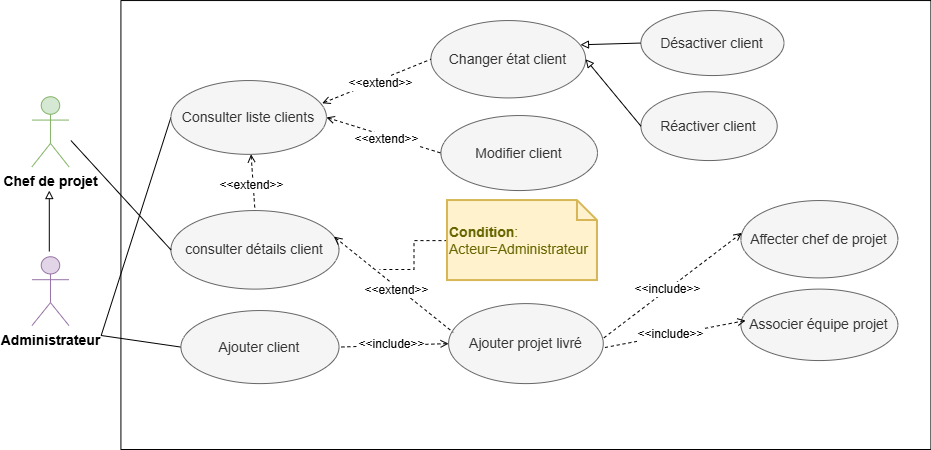
\includegraphics[width=0.8\textwidth,keepaspectratio]{Images/gerer client.drawio.png}
\caption{Raffinement de cas d'utilisation « Gérer clients »}
\label{fig:gerer_clients}
\end{figure}

\subsubsection{Description textuelle de cas d'utilisation « Consulter liste clients »}

\begin{table}[H]
\centering
\footnotesize
\renewcommand{\arraystretch}{1}
\caption{Description textuelle « Consulter liste clients »}
\begin{tabular}{|p{4.5cm}|p{12cm}|}
\hline
\textbf{Nom du cas d'utilisation} & Consulter liste clients \\
\hline
\textbf{Acteurs} & Administrateur, Chef de projet \\
\hline
\textbf{Préconditions} & L'utilisateur est authentifié\newline L'utilisateur possède la permission de consulter les clients\\
\hline
\textbf{Postconditions} & Liste des clients affichée\\
\hline
\textbf{Scénario principal} & 
\begin{minipage}[t]{\linewidth}
\begin{enumerate}[label=\arabic*., leftmargin=*]
\item L'utilisateur accède à la section "Clients".   
\item Le système affiche les clients sous forme de grille (par défaut).
\item L'utilisateur peut basculer entre trois modes d'affichage : grille, liste, ou vue par société.
\item L'utilisateur recherche un client en saisissant des informations clés dans la barre de recherche ou par des boutons de filtre (par statut, par secteur d'activité). 
\item Le système filtre les résultats.
\end{enumerate}
\vspace{2pt}
\end{minipage} \\
\hline
\textbf{Scénarios alternatifs} & \begin{itemize}[nosep,leftmargin=0.8cm,topsep=0pt,itemsep=2pt, label=$\bullet$]
\item L'utilisateur sélectionne la vue "Par société" pour regrouper les clients par société et visualiser les contacts associés à chaque société.
\item L'utilisateur clique sur le bouton « Exporter » pour télécharger la liste des clients (CSV, Excel).
\item L'utilisateur clique sur le bouton « Importer » pour ajouter plusieurs clients via un fichier (CSV, Excel).
\end{itemize} \\
\hline
\end{tabular}
\end{table}
\vspace{-0.3cm}

\subsubsection{Description textuelle de cas d'utilisation « Ajouter client »}

\begin{table}[H]
\centering
\footnotesize
\renewcommand{\arraystretch}{1}
\caption{Description textuelle « Ajouter client »}
\begin{tabular}{|p{4.5cm}|p{12cm}|}
\hline
\textbf{Nom du cas d'utilisation} & Ajouter un client \\
\hline
\textbf{Acteurs} & Administrateur \\
\hline
\textbf{Préconditions} & 
L'utilisateur est authentifié.\newline
L'utilisateur possède la permission de créer des clients. \newline
La liste des clients est accessible.\\
\hline
\textbf{Postconditions} & 
Le client est créé et enregistré dans le système. \newline
Le profil client associé est initialisé. \newline
Un message de confirmation est affiché. \\
\hline
\textbf{Scénario principal} & 
\begin{minipage}[t]{\linewidth}
\begin{enumerate}[label=\arabic*., leftmargin=*]
\item L'administrateur clique sur le bouton « Nouveau client ».
\item Le système affiche le formulaire de création.
\item L'administrateur saisit les informations du client : prénom, nom, e-mail et autres données requises.
\item L'administrateur renseigne ou sélectionne la société associée au client.
\item Si nécessaire, l'administrateur complète les informations de la société : nom, adresse, secteur d'activité et téléphone.
\item Le système peut récupérer automatiquement le logo de la société à partir d'une source externe, ainsi que l'adresse via un service de géocodage, si ces fonctionnalités sont activées.
\item L'administrateur valide le formulaire en cliquant sur « Créer le client ».
\item Le système vérifie la validité des données et l'unicité de l'e-mail.
\item Le système crée le client et associe son profil dans la base de données.
\item Le système envoie un e-mail de confirmation ou de bienvenue si cette fonctionnalité est prévue.
\item Le système affiche un message de succès et met à jour la liste des clients.
\end{enumerate}
\vspace{2pt}
\end{minipage} \\
\hline
\textbf{Scénarios alternatifs} & 
\begin{itemize}[nosep,leftmargin=0.8cm,topsep=0pt,itemsep=2pt, label=$\bullet$]
\item L'administrateur ajoute manuellement le logo de la société au lieu d'utiliser la récupération automatique.
\item L'administrateur associe le client à une société existante déjà enregistrée.
\item L'administrateur saisit manuellement l'adresse de la société lorsque la suggestion automatique du géocodage ne correspond pas.
\item L'administrateur complète plus tard certaines informations facultatives du client.
\end{itemize} \\
\hline
\textbf{Scénarios d'exception} & 
\begin{itemize}[nosep,leftmargin=0.8cm,topsep=0pt,itemsep=2pt, label=$\bullet$]
\item Un champ obligatoire est vide ou contient une valeur invalide.
\item L'adresse e-mail saisie est déjà utilisée par un autre utilisateur.
\item Le système rencontre une erreur lors de l'enregistrement du client.
\item L'administrateur tente de quitter le formulaire alors que des données ont déjà été saisies.
\end{itemize} \\
\hline
\end{tabular}
\end{table}
\vspace{-0.3cm}

% \subsubsection{Description textuelle de cas d'utilisation « Modifier client »}

% \begin{table}[H]
% \centering
% \footnotesize
% \renewcommand{\arraystretch}{1}
% \caption{Description textuelle « Modifier client »}
% \begin{tabular}{|p{4.5cm}|p{12cm}|}
% \hline
% \textbf{Nom du cas d'utilisation} & Modifier client \\
% \hline
% \textbf{Acteurs} & Administrateur \\
% \hline
% \textbf{Préconditions} & L'utilisateur est authentifié\newline L'utilisateur possède la permission de modifier les clients\newline Liste des clients affichée\\
% \hline
% \textbf{Postconditions} & Le client est modifié\\
% \hline
% \textbf{Scénario principal} & \begin{minipage}[t]{\linewidth}
% \begin{enumerate}[label=\arabic*., leftmargin=*]
% \item L'administrateur consulte la fiche du client choisi.                 
% \item L'administrateur clique sur le bouton (Modifier).                                                       
% \item Le système affiche le formulaire de modification.  
% \item L'administrateur modifie les informations souhaitées. 
% \item L'administrateur clique sur le bouton (Enregistrer).
% \item Le système met à jour les informations du client.
% \item Le système affiche le message de succès.
% \end{enumerate}
% \vspace{2pt}
% \end{minipage} \\
% \hline
% \textbf{Scénarios d'exception} & \begin{itemize}[nosep,leftmargin=0.8cm,topsep=0pt,itemsep=2pt, label=$\bullet$] 
% \item L'administrateur saisit un e-mail déjà utilisé par un autre utilisateur.
% \item L'administrateur tente de modifier un client ayant des contrats actifs sans validation.
% \end{itemize} \\
% \hline
% \end{tabular}
% \end{table}
% \vspace{-0.8cm}

\subsubsection{Description textuelle de cas d'utilisation « Consulter profil client »}

\begin{table}[H]
\centering
\footnotesize
\renewcommand{\arraystretch}{1}
\caption{Description textuelle « Consulter profil client »}
\begin{tabular}{|p{4.5cm}|p{12cm}|}
\hline
\textbf{Nom du cas d'utilisation} & Consulter profil client \\
\hline
\textbf{Acteurs} & Administrateur, Chef de projet, Client (son propre profil) \\
\hline
\textbf{Préconditions} & L'utilisateur est authentifié\newline L'utilisateur possède la permission de consulter les profils clients ou consulte son propre profil\newline Pour Chef de projet : le client doit être associé à au moins un de ses projets\\
\hline
\textbf{Postconditions} & Profil client consulté\\
\hline
\textbf{Scénario principal} & 
\begin{minipage}[t]{\linewidth}
\begin{enumerate}[label=\arabic*., leftmargin=*]
\item L'utilisateur accède au profil du client.
\item Le système affiche les informations personnelles et société.
\item Le système affiche les statistiques et éléments accessibles selon le rôle de l'utilisateur.
\item L'utilisateur peut naviguer vers les éléments disponibles (projets, demandes, tickets, documents).
\end{enumerate}
\vspace{2pt}
\end{minipage} \\
\hline
\textbf{Restrictions d'accès} & 
\begin{minipage}[t]{\linewidth}
\begin{itemize}[nosep,leftmargin=0.8cm,topsep=0pt,itemsep=2pt, label=$\bullet$]
\item Administrateur : accès complet (contrats, projets, demandes, tickets, notes privées, documents).
\item Chef de projet : accès limité aux projets où il est assigné et aux demandes/tickets liés à ces projets uniquement.
\item Client : accès à son propre profil, ses projets, demandes et tickets.
\end{itemize}
\vspace{2pt}
\end{minipage} \\
\hline
\textbf{Scénarios alternatifs} & \begin{itemize}[nosep,leftmargin=0.8cm,topsep=0pt,itemsep=2pt, label=$\bullet$]
\item L'utilisateur exporte les informations du profil en PDF.
\item L'utilisateur clique sur "Contacter" pour envoyer un e-mail ou un message via la messagerie interne de l'application.
\item L'utilisateur clique sur l'adresse de la société pour visualiser sa localisation sur une carte interactive.
\item L'administrateur ajoute une note privée sur le client.
\end{itemize} \\
\hline
\end{tabular}
\end{table}
\vspace{-0.3cm}

\subsubsection{Description textuelle de cas d'utilisation « Désactiver client »}

\begin{table}[H]
\centering
\footnotesize
\renewcommand{\arraystretch}{1}
\caption{Description textuelle « Désactiver un client »}
\begin{tabular}{|p{4.5cm}|p{12cm}|}
\hline
\textbf{Nom du cas d'utilisation} & Désactiver un client \\
\hline
\textbf{Acteurs} & Administrateur \\
\hline
\textbf{Préconditions} & L'utilisateur est authentifié\newline L'utilisateur possède la permission de désactiver les clients\newline Liste des clients affichée\newline Le client à désactiver doit être actuellement Actif\\
\hline
\textbf{Postconditions} & Le compte client est désactivé\\
\hline
\textbf{Scénario principal} & \begin{minipage}[t]{\linewidth}
\begin{enumerate}[label=\arabic*., leftmargin=*]
\item L'administrateur choisit un client dans la liste.                 
\item L'administrateur clique sur l'action (Désactiver).                                                     
\item Le système vérifie si le client possède des contrats actifs, des demandes en cours ou des tickets actifs.  
\item Le système affiche une boîte de dialogue de confirmation avec les détails des contrats, demandes et tickets actifs. 
\item L'administrateur confirme l'action.
\item Le système met à jour le statut du client.
\item Le système révoque les sessions actives (suppression des refresh tokens).
\item Le système envoie un e-mail automatique au contact principal du client pour l'informer de la désactivation.
\item Le système affiche le message de succès.
\end{enumerate}
\vspace{2pt}
\end{minipage} \\
\hline
\textbf{Scénarios d'exception} & \begin{itemize}[nosep,leftmargin=0.8cm,topsep=0pt,itemsep=2pt, label=$\bullet$] 
\item L'administrateur tente de désactiver un client qui possède des contrats actifs sans les clôturer.
\item L'administrateur tente de désactiver un client ayant des demandes en attente de traitement.
\item L'administrateur tente de désactiver un client ayant des tickets actifs non résolus.
\end{itemize} \\
\hline
\textbf{Scénarios alternatifs} & L'administrateur clôture les contrats, traite les demandes et résout les tickets avant la désactivation. \\
\hline
\end{tabular}
\end{table}
\vspace{-0.3cm}

\subsubsection{Description textuelle de cas d'utilisation « Réactiver client »}

\begin{table}[H]
\centering
\footnotesize
\renewcommand{\arraystretch}{1}
\caption{Description textuelle « Réactiver un client »}
\begin{tabular}{|p{4.5cm}|p{12cm}|}
\hline
\textbf{Nom du cas d'utilisation} & Réactiver un client \\
\hline
\textbf{Acteurs} & Administrateur \\
\hline
\textbf{Préconditions} & L'utilisateur est authentifié\newline L'utilisateur possède la permission de réactiver les clients\newline Le compte client doit être désactivé\\
\hline
\textbf{Postconditions} & Le compte client est réactivé\\
\hline
\textbf{Scénario principal} & \begin{minipage}[t]{\linewidth}
\begin{enumerate}[label=\arabic*., leftmargin=*]
\item L'administrateur consulte la liste des clients désactivés.
\item L'administrateur sélectionne un client à réactiver.
\item L'administrateur clique sur l'action (Réactiver le compte).
\item Le système affiche une confirmation.
\item L'administrateur confirme l'action.
\item Le système réactive le compte.
\item Le système envoie un e-mail au client.
\item Le système affiche le message de succès.
\end{enumerate}
\vspace{2pt}
\end{minipage} \\
\hline
\textbf{Scénarios d'exception} & Le client est déjà actif. \\
\hline
\end{tabular}
\end{table}
\vspace{-0.3cm}


\newpage

% ─────────────────────────────────────────────────────────────────────────────
% SECTION 3 : CONCEPTION
% ─────────────────────────────────────────────────────────────────────────────

\section{Diagramme de classes de deuxiéme sprint}

\section{Diagramme de séquence}
\subsection{Diagramme de séquences du cas d'utilisation « Demande Résiliation »}

\begin{figure}[H]
        \centering
        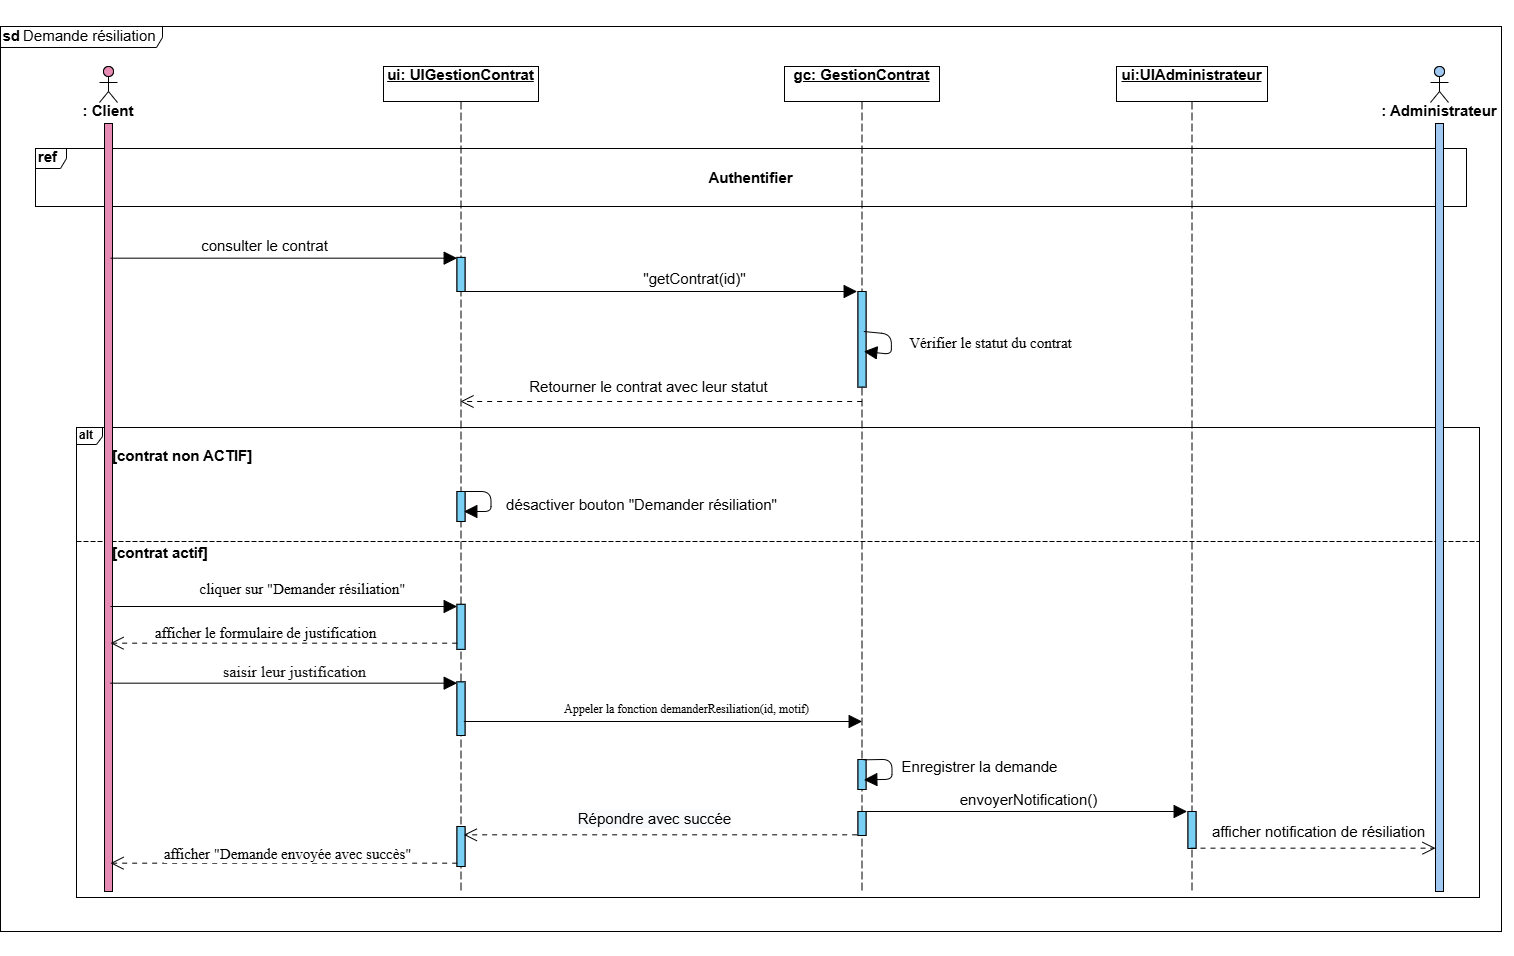
\includegraphics[width=0.7\textwidth,keepaspectratio]{Images/Diagramme de sequence Demande Resiliation.png}
        \caption{Diagramme de séquence du cas d'utilisation «  Demande Résiliation »}
        \label{fig:Diagramme de sequence Demande Resiliation}
\end{figure}
\subsection{Diagramme de séquences du cas d'utilisation « Résilier contrat »}

\begin{figure}[H]
        \centering
        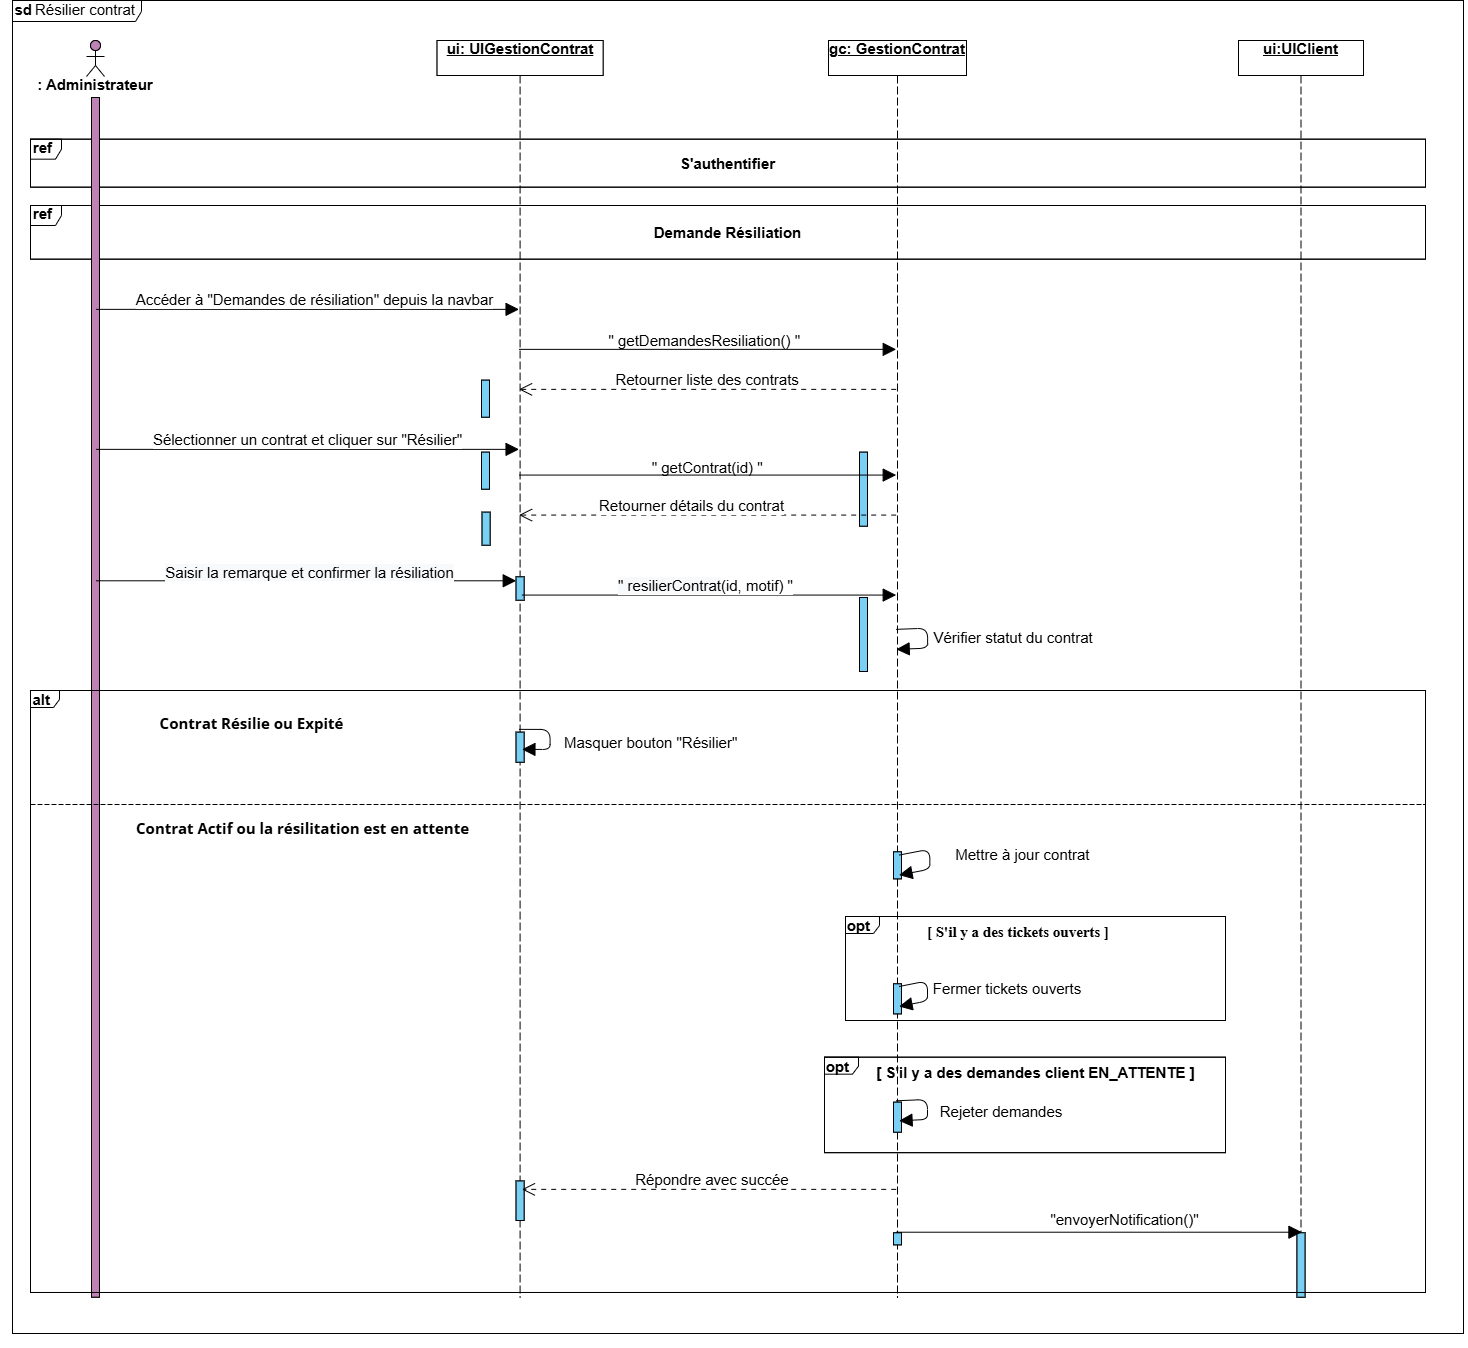
\includegraphics[width=0.7\textwidth,keepaspectratio]{Images/Diagramme de sequence de resilier contrat.png}
        \caption{Diagramme de séquence du cas d'utilisation « Résilier contrat »}
        \label{fig:Diagramme de sequence de resilier contrat}
\end{figure}

\newpage

% ─────────────────────────────────────────────────────────────────────────────
% SECTION 4 : RÉALISATION
% ─────────────────────────────────────────────────────────────────────────────

\section{Réalisation}
\label{sec:realisation_sprint2}

\subsection{Architecture technique}

Cette section présentera l'architecture technique mise en place pour le Sprint 2, incluant les modules de gestion des clients, projets et contrats.

\textit{[À compléter avec les détails d'implémentation]}

\subsection{Interfaces utilisateur}

Cette section présentera les principales interfaces développées durant le Sprint 2.

\textit{[À compléter avec les captures d'écran]}

\newpage

% ─────────────────────────────────────────────────────────────────────────────
% SECTION 5 : TESTS
% ─────────────────────────────────────────────────────────────────────────────

\section{Tests}
\label{sec:tests_sprint2}

\subsection{Tests unitaires}

Cette section présentera les tests unitaires réalisés pour valider les fonctionnalités du Sprint 2.

\textit{[À compléter avec les résultats des tests]}

\subsection{Tests d'intégration}

Cette section présentera les tests d'intégration effectués pour s'assurer du bon fonctionnement global du système.

\textit{[À compléter avec les résultats des tests]}
